\documentclass{article}
\usepackage[affil-it]{authblk}
\usepackage{graphicx}
\usepackage{longtable}
\usepackage{float} 
\usepackage{amsmath}

\title{Risk of being killed by police use-of-force in the U.S. by age, race/ethnicity, and sex}
\author{Frank Edwards, Hedwig Lee, and Michael Esposito}
\correspondingauthor{Frank Edwards.\\E-mail: frank.edwards@rutgers.edu}

\begin{document}

\maketitle


\section*{Introduction: Rare events and unofficial data}

The analyses in this paper seek to simultaneously address two significant methodological challenges. The first is the relative rarity of police-involved killings for many age-sex-race specific subgroups with small national populations. The second is the absence of valid official data. 

First, Police killings are a relatively rare event for many race-age-sex specific subgroups. For example, we estimate that Asian/Pacific Islander women between the ages of 50 and 54 are killed by police at a rate of about $0.04$ per $100000$ person-years. In 2017, the American Community Survey reports a population of Asian/Pacific-Islander women between the ages of 50 and 54 of $666102$. At our estimated rate of police use-of-force killings, we expect to observe an average of about 0.3 deaths per year in this age group. Between 2013 and 2017, we observe only one death in this age-race-sex group. Relying on any single year for life table estimates would produce a misleading estimate for age-specific risk, with a single-year estimated rate varying between zero and $0.15$ per $100000$ depending on the presence or absence of a death in that year. By including multiple years of valid data and using statistical models, we are able to incorporate dramatically more information to estimate risk. However, by doing so, we assume that differences in risk across groups over time remain relatively stable. Temporal trends can be directly modeled as a source of uncertainty. We rely on multilevel models and Bayesian simulation to directly incorporate multiple sources of uncertainty to more accurately estimate mortality risk. We describe these methods in more detail below.

Second, there are currently no nationally comprehensive official sources of data on police-involved killings. The Bureau of Justice Statistics acknowledged the limitations of their Arrest-Related Deaths data collection effort, and ceased data collection in 2014 \cite{banks2016arrest}. The National Vital Statistics System (NVSS), the nation's key source of mortality data is known to undercount law enforcement related deaths \cite{Feldman2017Quantifying}. The National Violent Death Reporting System (NVDRS) has far better coverage of police-involved deaths than does NVSS \cite{conner2019validating}, but currently lacks the geographic and temporal coverage needed to generate national risk estimates. Despite calls for better data on police-involved deaths \cite{Krieger2015Police}, government agencies have systematically failed to design and implement such a system to track officer-involved killings, or more generally, officer use-of-force. Journalists and independent researchers have stepped into this gap. Following the rise of the Black Lives Matter movement and increasing attention paid to police killings of people of color in the mid 2010s, multiple projects emerged to use public records and media reports to systematically document police violence. However, these unofficial data have important limitations. We describe these limitations and assess the validity of the data relative to the partial data available from the NVSS below.

\section*{Assessing the validity of unofficial data on police-involved deaths}

Among these novel data collection efforts, Fatal Encounters has the broadest temporal scope and inclusion criteria for police-involved deaths. Where other efforts have focused exclusively on shootings or a narrow subset of years, Fatal Encounters seeks to include all cases in which police were in any way involved in a death of a civilian between January 1, 2000 and the present, with the exception of deaths occurring in custody (that is after an arrestee has been formally booked into a jail or other detention facility). Below, we consider the validity of counts derived from Fatal Encounters over time, and evaluate the validity of individual variables in FE. To do so, we largely rely on comparisons to deaths recorded as police-involved in the NVSS. While NVSS is known to significantly undercount these cases \cite{Feldman2017Quantifying}, it provides some information about trends over time and the racial composition of deaths that we can use to inspect any serious deviations from the patterns we observe in Fatal Encounters.

\subsection*{Comparing trends in NVSS and Fatal Encounters}

The National Vital Statistics System provides a potential source for evaluating the external validity of Fatal Encounters data. ``Legal intervention'' is included among the ICD-10 codes for causes of death in NVSS. Prior research has established that NVSS systematically undercounts officer-involved deaths \cite{Feldman2017Quantifying}. However, if we assume that there has been no change in the probability that officer-involved deaths are coded as ``legal intervention'' in NVSS over time, the observable time series trends in NVSS should be correlated with the true unobserved time series of police-involved deaths. With this assumption, we evaluate the time series of NVSS police-involved deaths and Fatal Encounters officer use-of-force deaths to explore whether FE consistently tracks the NVSS trend over time and gain insight into temporal trends in the risk of police-involved death. We display this time series in Figure \ref{fig:countTS}. Because NVSS counts are significantly lower than FE counts, we provide a time series transformed to a proportional change in counts of deaths relative to the count of deaths in 2000 in each dataset in Figure \ref{fig:pctTS} to enable direct comparison of the two trends on a common scale. 

\begin{figure}
	\centering
	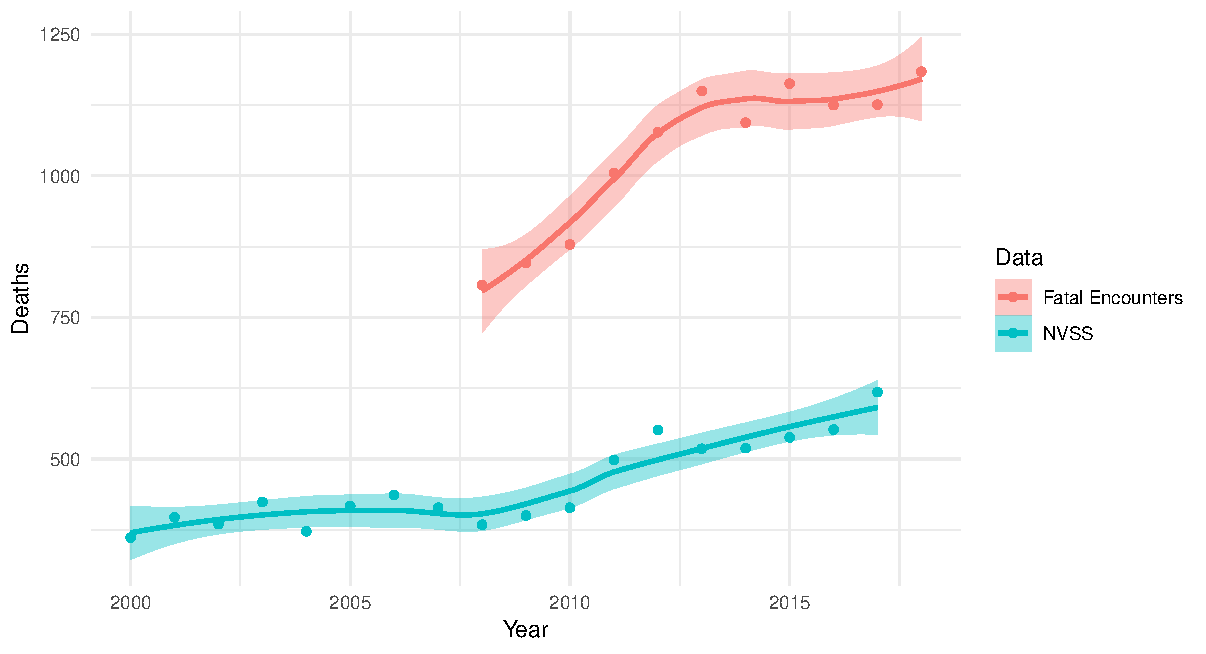
\includegraphics[width = \linewidth]{vis/nvss_fe_ts.pdf}
	\caption{Deaths due to officer use of force recorded in Fatal Encounters and NVSS 2000 to 2018}
	\label{fig:countTS}
\end{figure}

\begin{figure}
	\centering
	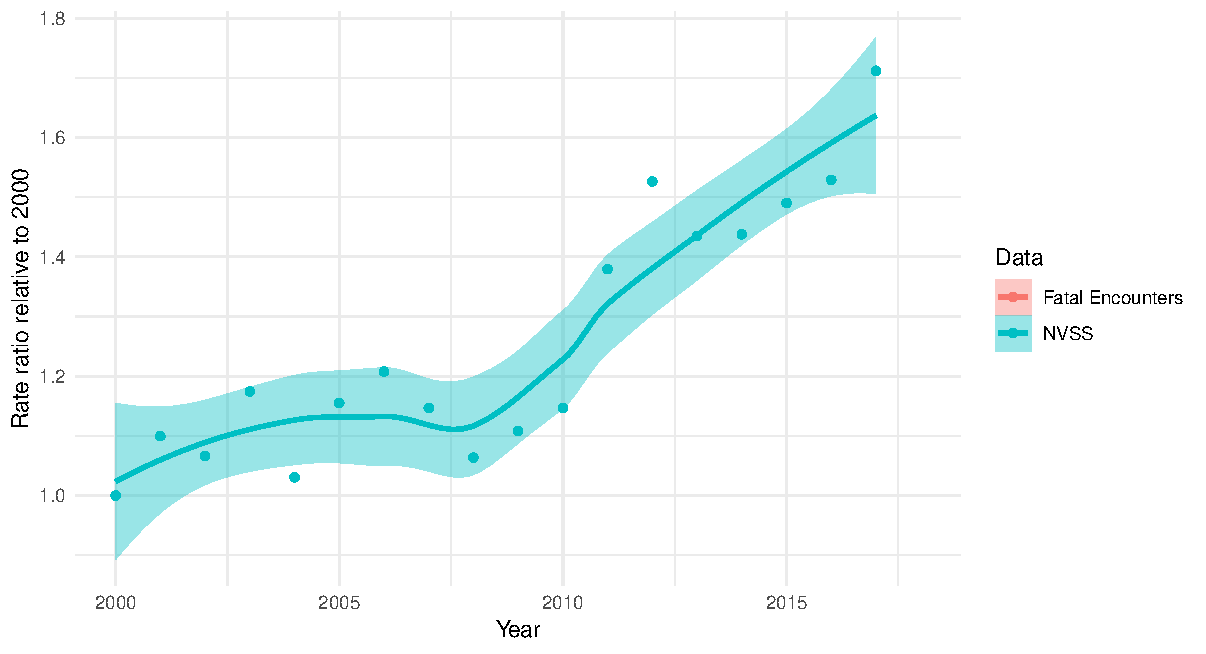
\includegraphics[width = \linewidth]{vis/nvss_fe_pct.pdf}
	\caption{Proportional change in reported deaths in NVSS and Fatal Encounters since 2000}
	\label{fig:pctTS}
\end{figure}

Figures \ref{fig:countTS} and \ref{fig:pctTS} show that counts of deaths reported in NVSS remained relatively stable between 2000 and 2010. During this time, rates fluctuated between 1.0 and 1.2 times the count of officer-involved deaths reported in 2000. Between 2011 and 2017 (the most recent available data), the count of cases in the data increased substantially. In 2017, there were about 1.7 times more legal intervention deaths reported in NVSS than there were in 2000. 

Fatal Encounters exhibits a relatively stable positive trend between 2000 and 2018. The magnitude of growth in cases recorded in FE over time is higher than for NVSS; for 2018, FE records about 2.3 times more deaths than it records for 2000. While this evidence is far from definitive, trends in the proliferation of internet access and the NVSS time series suggest that undercounts in Fatal Encounters due to unavailable online news records of officer-involved deaths likely decreased over time until approximately 2007. The shape of trends in Fatal Encounters and NVSS become more tightly linked between 2008 and 2017. 

\begin{figure}
	\centering
	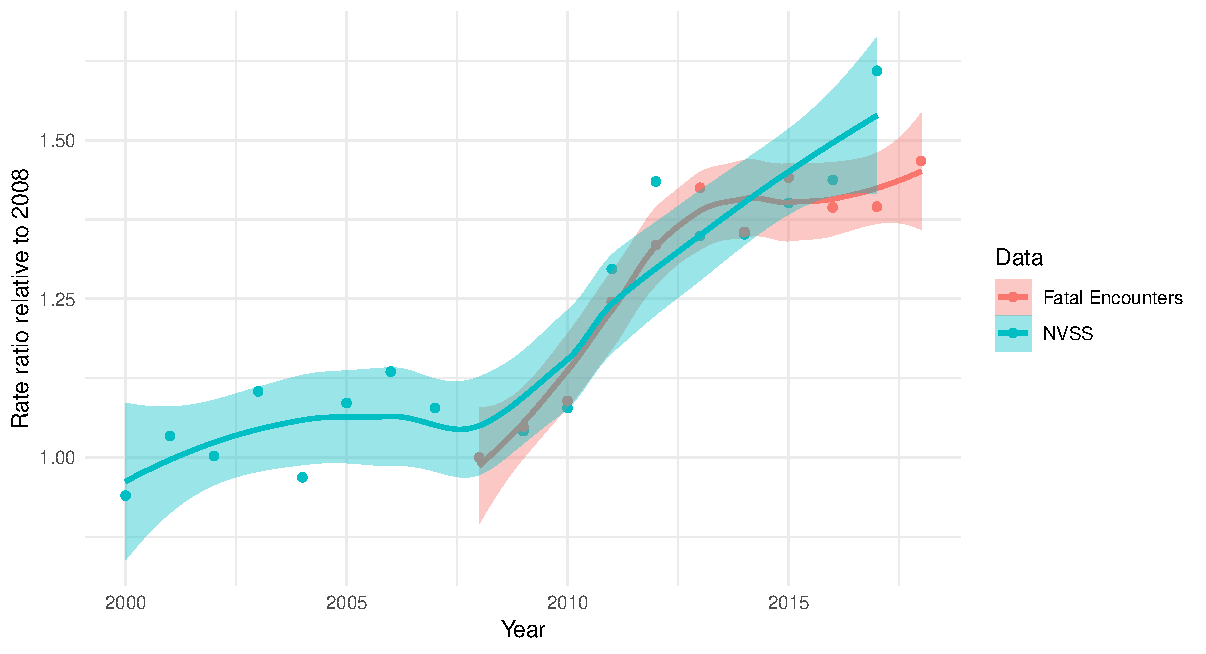
\includegraphics[width = \linewidth]{vis/nvss_fe_pct_08.pdf}
	\caption{Proportional change in reported deaths in NVSS and Fatal Encounters since 2008}
	\label{fig:pct_08}
\end{figure}

Figure \ref{fig:pct_08} rescales both time series to display proportional changes in case counts relative to the observed counts for 2008. This figure strongly suggests that the trends in NVSS and Fatal Encounters converge after 2008. It may be fruitful in future research to estimate the magnitude of undercoverage in FE using secondary data like NVSS. Based on this analysis, we assume that undercoverage in Fatal Encounters becomes less pronounced after 2007, and focus our analyses on cases after 2008. Because of the quality of race / ethnicity data in FE, we further restrict the time series to 2013 - 2018, discussed in more detail below.

\section*{Race/ethnicity data in Fatal Encounters}

Fatal Encounters codes decedent race with the mutually exclusive values: African American / Black; Asian / Pacific Islander; European-American / White; Hispanic / Latino; Middle Eastern; Native American / Alaskan; and Race unspecified. Ethnicity is not coded separately from race, so no distinctions among ethnic groups (i.e. Black and non-Black Latinx people) are possible using these data. We preserve these categories in all analyses, with the exception of Middle Eastern, which we recode to "White" based on census racial classifications to match population data. 

Fatal Encounters codes race/ethnicity opportunistically based on a series of potential data sources. When available, official records or news reports that explicitly identify a victim's race or ethnicity are used. However, such identifications are rare in news reports, which typically adhere to style guidelines limiting the use of racial or ethnic categories in their reporting. When explicit identifications are unavailable, Fatal Encounters researchers combine information and photos from original news reports, obituaries, or social media profiles to make qualitative assessments of a victim's race and ethnicity. 

While researcher perceived race based on cues such as skin tone, name, and manner of dress is informative, it has distinct limits. Researcher perceived race may correlate with the perception of a victim's race held by the officer involved in the focal fatal encounter. Perceptions of an individual's racial or ethnic identity, rather than an individual's self-identification, may activate biases or scripts that structure the officer's interaction with the victim. However, the social and cultural background and information available to either the officer or researcher may differ in ways that lead to different appraisals of victim race/ethnicity. An individual's self-identified race/ethnicity may also differ in important ways from an officer or researcher's perception of their race/ethnicity. This is particularly relevant for multi-racial or multi-ethnic victims, for American Indian / Alaska Native victims, and for Latinx victims. 

Like overall counts of cases in Fatal Encounters, earlier years recorded in the data are likely subject to diminished quality due to the gradual development of internet news coverage, the timing of the development of major social media platforms, and the development of online obituary services, all of which made photos of individuals more widely available. We show a time series of the proportion of cases missing race/ethnicity data in FE in Figure \ref{fig:missing_race_ts}.

\begin{figure}
	\centering
	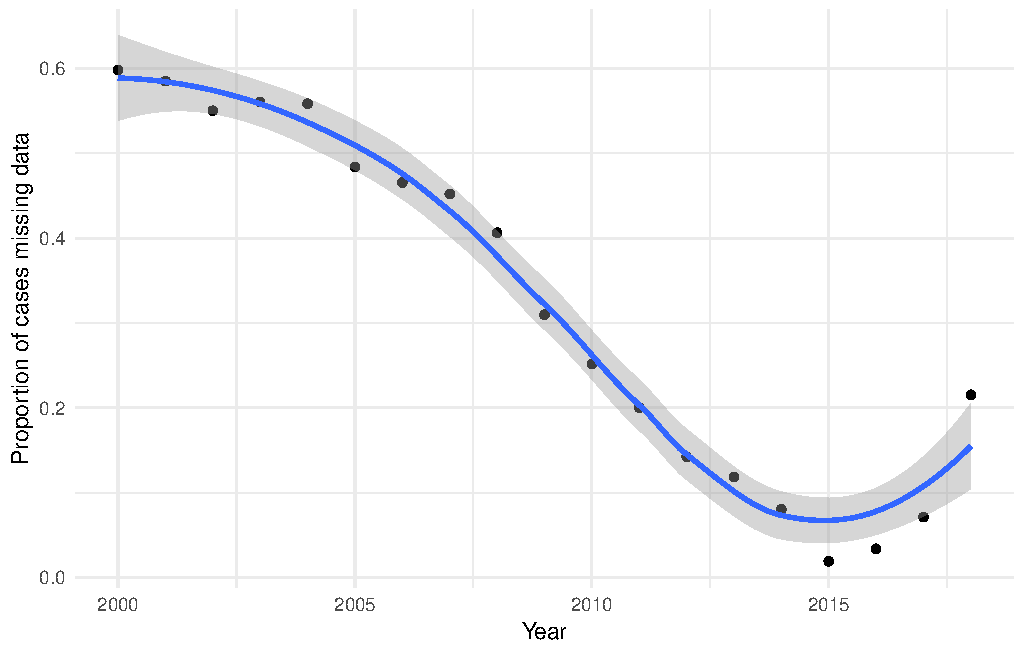
\includegraphics[width=\linewidth]{vis/prop_missing_race.pdf}
	\caption{Proportion of use-of-force cases missing data on race/ethnicity in Fatal Encounters, 2000 - 2018}
	\label{fig:missing_race_ts}
\end{figure}

About 60 percent of use-of-force cases documented for 2000 are missing data on race/ethnicity. This proportion decreases steadily toward a minimum of about two percent of cases in 2015, followed by a gradual increase in recent years. Fatal Encounters researchers return to cases previously coded only based on news reports to conduct additional searches for obituaries published after the initial incident. In conversation with the authors, Fatal Encounters indicated that missing race/ethnicity data for 2018 and 2019 should be reduced once researchers conduct obituary searches for cases ocurring in these years.

\subsection*{Comparing Fatal Encounters to NVSS data on race/ethnicity}

To evaluate the validity of Fatal Encounters race / ethnicity data, we again turn to the NVSS. If we assume that each racial / ethnic group has a similar probability of being recorded as a ``legal intervention'' death, conditional on being killed by police, then the relative case composition of legal intervention deaths in NVSS can be used to detect systematic bias in Fatal Encounters' race/ethnicity data. Research suggests that race is not likely affecting the probability of cases being recorded as legal intervention deaths in NVSS \cite{Feldman2017Quantifying}. Below, we present the composition of Fatal Encounters cases prior to any missing data imputation procedures to ensure direct comparisons between the data recorded in each source. 

\begin{figure}
	\centering
	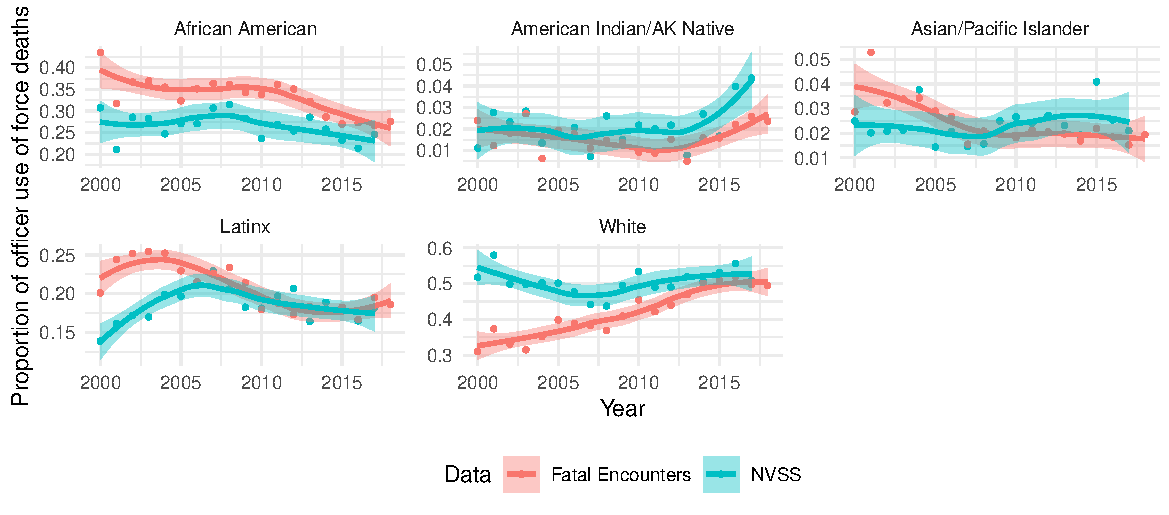
\includegraphics[width = \linewidth]{vis/fe_nvss_race_compare_na_rm.pdf}
	\caption{Proportion of cases in NVSS and Fatal Encounters by race, excluding cases missing race/ethnicity data, 2000 - 2018. Note that y-axis scales vary for each plot}
	\label{fig:compare_missing_na_rm}
\end{figure}

Figure \ref{fig:compare_missing_na_rm} shows the case composition by race/ethnicity excluding cases missing race/ethnicity data from the total case count in the proportion denominator. Note that there are no ``legal intervention'' cases missing race/ethnicity data in the NVSS. Both Fatal Encounters and NVSS record similar proportions of Asian / Pacific Islander victims. Until 2010, FE and NVSS record similar shares of American Indian victims, but NVSS records a greater share of American Indian / Alaska Native cases than does FE after 2010. Latinx victims made up a greater share of Fatal Encounters cases prior to 2008, but Latinx compositions appear similar across the datasets between 2008 and 2017. African Americans make up a consistently larger share of the case composition in Fatal Encounters than in NVSS. Among non-missing cases, Black victims composed between 40 and 28 percent of the caseload between 2000 and 2018. White victims ranged between 30 and 50 percent of the cases in Fatal Encounters, while NVSS consistently reports a white case composition of between 45 and 60 percent. The difference in case compositions between FE and NVSS for both white and Black victims diminishes between 2010 and 2017.

Fatal Encounters researchers note that they have most confidence in their race/ethnicity data for data years after 2013. Between 2013 and 2017 (the latest available NVSS data), Fatal Encounters' African American case composition was between 8 and 28 percent higher than NVSS, the American Indian / Alaska Native case composition was between 6 and 44 percent lower than NVSS, the Asian Pacific Islander case composition was between 12 and 46 percent lower than NVSS, the Latinx caseload was between 5 percent lower and 12 percent higher than NVSS, and the white case composition was between 1 and 9 percent lower than NVSS. 

It is important to note that FE records as many or more deaths than NVSS for nearly all racial / ethnic groups during this time period. Between 2013 and 2017, FE records $2549$ more cases than does NVSS (excluding $364$ cases missing race ethnicity data). Between 2008 and 2012, FE records more cases than does NVSS for all groups other than American Indian / Alaska Natives. In 2008, 2010, and 2011, FE records 3 fewer American Indian / Alaska Native deaths than does NVSS. In 2009 and 2012, FE records 2 more deaths than does NVSS. 

This comparison shows that FE racial/ethnic case compositions have some divergence from NVSS case compositions, and that these differences ar most pronounced for African Americans, American Indians, and Asian / Pacific Islanders. Despite these divergences, FE is generally recording dramatically more cases for each subgroup than is NVSS. Relative to NVSS, observed counts in Fatal Encounters are not negatively biased for any subgroup, with the potential exception of American Indian / Alaska Natives in years prior to 2012. Mortality rate ratios based solely on the observed data may be biased when relying on FE data if NVSS race data is unbiased. Future researchers may consider conducting a systematic audit of FE race/ethnicity coding to evaluate the interrater reliability of FE coding decisions for race / ethnicity. 

\section*{Multiple imputation of missing data in Fatal Encounters}

Table \ref{tab:pct_var} shows the percent of cases missing data on each variable in Fatal Encounters between 2013 and 2018 for all causes of death, including suicides and non-use-of-force related deaths. Because we have reason to believe that case counts are censored in earlier years of the data and because FE reports low confidence in race / ethnicity data prior to 2012, we exclude observations from 2000 to 2012 in imputation models. About 1.8 percent of cases are missing data on victim age, about 0.1 percent are missing data on victim sex, and about 9 percent are missing data on victim race. 

Our approach to missing data seeks to accurately describe uncertainty in mortality estimates by directly accounting for error driven by missing data, as well as providing rate estimates that are not negatively biased through the list-wise deletion of cases missing data on particular variables.

% latex table generated in R 3.5.2 by xtable 1.8-3 package
% Wed Mar  6 19:46:07 2019
\begin{table}[ht]
\centering
\begin{tabular}{rrrr}
  \hline
Age & Sex & Race & Cause of death \\ 
  \hline
3.050 & 0.349 & 21.200 & 0.006 \\ 
   \hline
\end{tabular}
\caption{Focal variables missing values in Fatal Encounters, percent of cases 2008 - 2018} 
\label{tab:pct_var}
\end{table}


To address missing data, we draw multiple imputations of missing values based on models including information on the year of death, victim age, victim sex, victim race, the cause of death, the racial composition of the county in which the victim was killed, and the probability of a victim's race/ethnicity conditional on victim surname compiled from Census surname lists by Imai and Khana \cite{imai2016improving}. Sensitivity analyses exploring the predictive validity of county, tract and block-group-level demographics suggested that county-level demographics maximized model classification validity. This is perhaps due to the fact that geodata recorded in Fatal Encounters records the location of death, and many victims recorded in Fatal Encounters did not die at home. 

Multiple imputation enables us to model uncertainty in the composition of cases in Fatal Encounters driven by missing data through the construction of uncertainty intervals derived from samples from our missing data models. These count estimates are by definition equal to or greater than those directly estimated from the observed data. However, by making the assumption that values are missing at random conditional on model predictors, we are able to provide additional precision in estimating the range within which actual mortality risk likely lies for each subgroup. We show the impacts of imputation on mortality risk estimates in Figure \ref{fig:na_rm}. For all groups, risk estimates based solely on imputed and observed data (not model predictions) yield estimates greater than or equal to values based on estimates from the observed data in which cases missing values are deleted. Lower bounds on our estimates after imputation are generally close to these list-wise deletion estimates. However, our imputation procedure enables a more realistic examination of uncertainty in risk by incorporating missing data as a source of measurement error.

\begin{figure}
	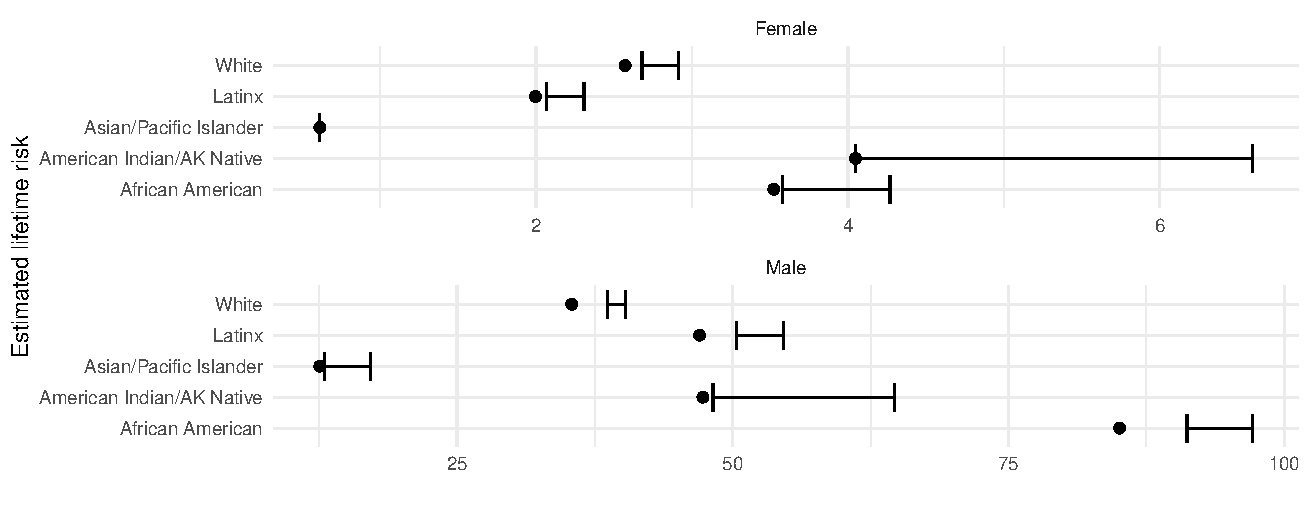
\includegraphics[width=\linewidth]{vis/imp_period_sensitivity.pdf}
	\caption{Sensitivity of risk estimates to missing data. Points indicate cumulative risk from Fatal Encounters 2013-2018 use of force deaths, excluding cases missing race/ethnicity data. Error bars indicate full interval of risk estimates using imputed values (not model simulations)}
	\label{fig:na_rm}
\end{figure}

\begin{figure}
	\centering
	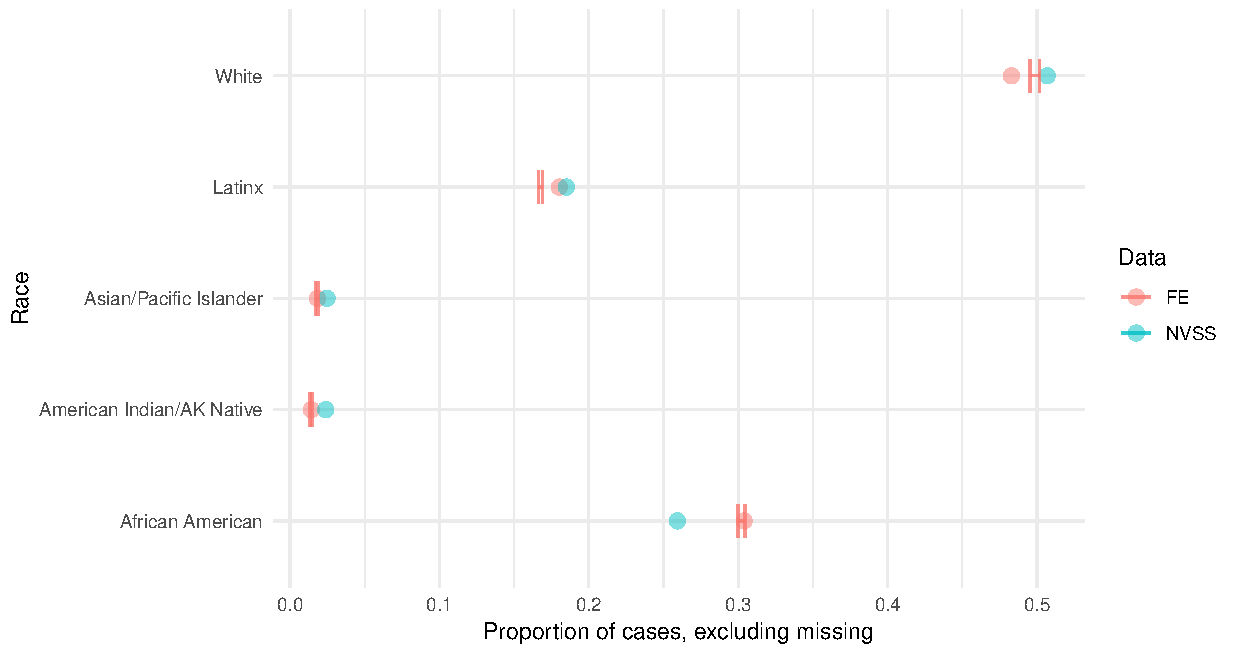
\includegraphics[width = \linewidth]{vis/race_impute_pct.pdf}
	\caption{Proportion of cases in observed Fatal Encounters and NVSS data (point) and range of imputed data (bar), 2013 - 2018}
	\label{fig:race_impute_pct}
\end{figure}

\begin{figure}
	\centering
	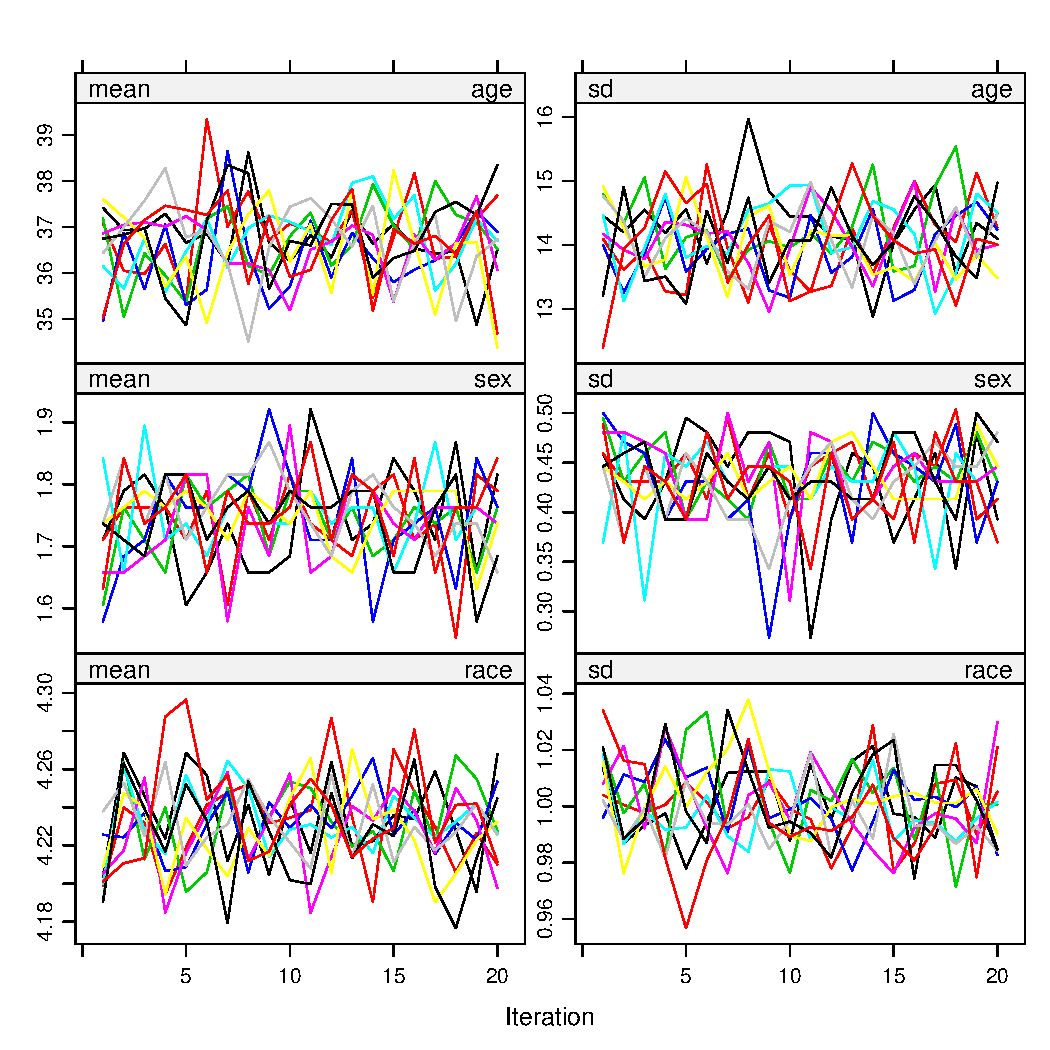
\includegraphics[width = \linewidth]{vis/imp_trace.pdf}
	\caption{Traceplot of mean and standard deviation of imputed variables}
	\label{fig:traceplot}
\end{figure}

Model predictions are generated using multiple imputation through chained equations \cite{buuren2010mice}. We construct 10 imputed datasets to ensure adequate coverage of uncertainty intervals for the race variable, which has a high number of missing cases in late years of the data. 

Figure \ref{fig:traceplot} shows the estimated mean and standard deviation of each imputed dataset (color) by variable across iterations, using an MCMC based approach to imputing predicted values in resulting datasets. The traceplots indicate model convergence, and appear free of any trends. 

We show the distribution of the imputed race/ethnicity variable relative to the observed data in Figure \ref{fig:race_impute_pct}. The solid points in this figure represent the observed proportion of cases in each group, and the bars represent the range of the imputed values. For American Indian, Asian, and Black people, the proportion of the observed FE data in each group is within the range of the imputed values. The distribution of the imputed data do not greatly differ than the distribution of the observed data for these groups. There is a greater share of Latinx victims in the observed data than there are in the imputed data, and there is a greater share of white victims in the imputed data than there are in the observed data. 

In the observed data (excluding missing cases), Latinx victims make up about 18 percent of the recorded cases. Our imputations suggest that they make up between 16.7 and 16.9 percent of all cases. White victims make up about 48 percent of the recorded cases in the observed data. Our imputations suggest they make up between 49.5 and 50.1 percent of all cases. 

This gap between imputed and observed proportions in Fatal Encounters is a function of the relationship between the probability of missingness and a victim's race/ethnicity. Our imputation models address this dependence by including two direct predictors of victim race/ethnicity; victim surname and racial/ethnic population composition in the county of death. 

To evaluate whether these predictors are correlated with missingness, we model the probability that a case is missing race/ethnicity data with a logistic regression. Selected parameter estimates from this model are displayed in Table \ref{tab:missing_reg}. 

% latex table generated in R 3.5.2 by xtable 1.8-3 package
% Wed Feb 27 15:47:58 2019
\begin{table}[H]
\centering
\begin{tabular}{lrr}
  \hline
Term & Estimate & SE \\ 
  \hline
County proportion American Indian & 0.20 & 0.45 \\ 
  County proportion Asian & -0.24 & 0.34 \\ 
  County proportion Black & -0.04 & 0.16 \\ 
  County proportion Hispanic & -0.96 & 0.16 \\ 
  Pr(White$|$Surname) & -1.06 & 0.54 \\ 
  Pr(Black$|$Surname) & -0.97 & 0.57 \\ 
  Pr(Hispanic$|$Surname) & -1.16 & 0.54 \\ 
  Pr(Asian$|$Surname) & -0.85 & 0.59 \\ 
   \hline
\end{tabular}
\caption{Relationships between county racial demographics,
         surnames and likelihood of missing race/ethnicity data in Fatal Encounters 2000 - 2018.
         Logistic regression with year intercepts, age slope, sex intercept, and
         cause of death intercept estimated but not displayed.} 
\label{tab:missing_reg}
\end{table}


Cases are less likely to be missing data when they are in counties with large Hispanic populations than when they occur in counties with smaller Hispanic populations. A surname with a high conditional probability of being Hispanic based on census records is also associated with a a lower probability of being missing. These relationships suggest that names and locations of death are associated with a higher likelihood of positive ethnic identification in Fatal Encounters, either through identifying features in initial reports, or through coder inference based on surname or other contextual information. Because Latinx victims are less likely to be missing in the observed data, their share of total reports in imputed data is somewhat lower.

\section*{Models of temporal variation in group-specific risk}

To systematically combine multiple years of FE data, we build Bayesian negative binomial regression models of police-involved deaths with year, race, sex and age as predictors. We use these models to predict group-specific risks of being killed by police for a year \textit{unobserved} in the data. Our prediction for a new year represents our best estimate of underlying police-homicide risk for each demographic group, synthesized from the available data. This approach incorporates temporal variation in risk across the 2013 - 2018 period as a source of uncertainty in our risk estimates. 

We assume -- and confirm, later, via model comparison tests -- that police-homicide risk varies jointly by age, sex and race. To appropriately incorporate time, which has a more ambiguous functional relationship with homicide risk, into our models, we first examine how police-homicides vary across years in the observed data.  

Figure \ref{fig:a1} displays the count of police-involved deaths for each sex and race group as a function of time. For most groups, the observed count of police involved deaths stays stable from 2013-2018. Mortality counts vary most notably among Latinas, with counts falling to lows in 2015 and 2016.

\begin{figure}
\center
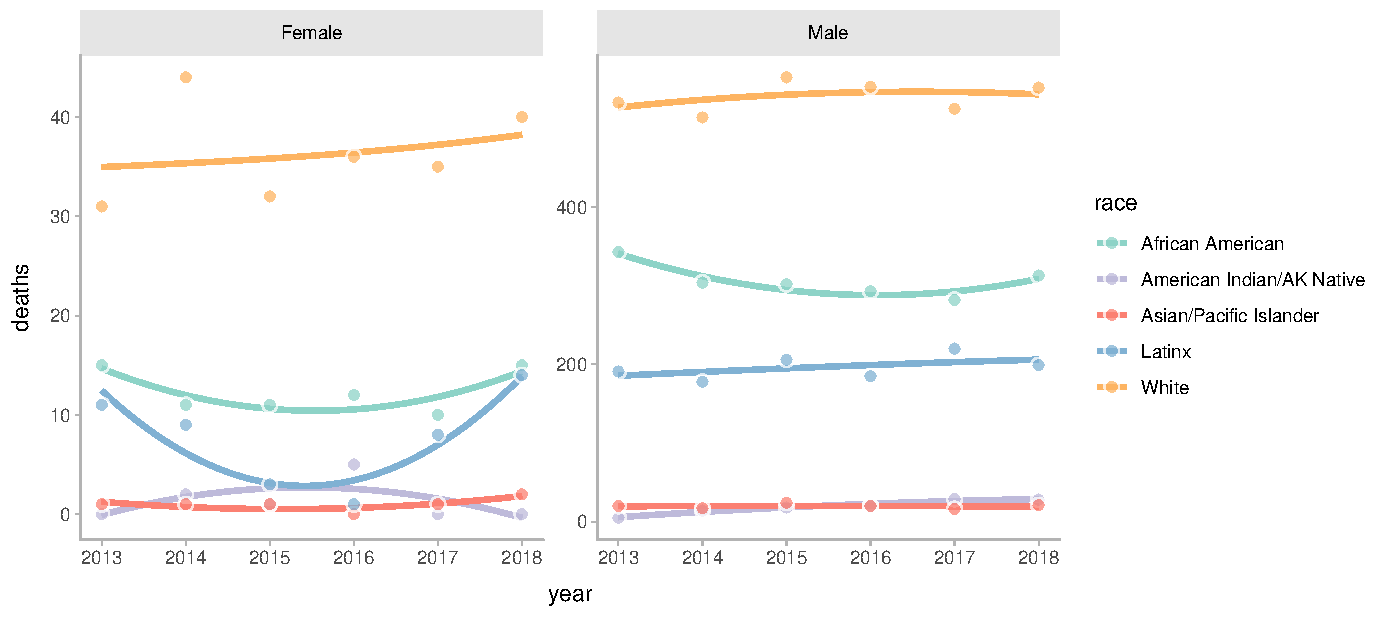
\includegraphics[width = \linewidth]{vis/fig_a1.pdf}
\caption{Observed count of police-involved deaths by race and sex, 2013-2018 with loess smooth}
\label{fig:a1}
\end{figure}

Next, Figures \ref{fig:a2} and \ref{fig:a3} display the observed relationship among age, race, sex and count of police-homicides within each year of the data. Among males, the age-specific risk of being killed by police is stable across years for all racial groups. Small, year based shifts in total deaths are apparent. For Black males, for example, the count of mortalities in 2013 is slightly higher the count of mortalities in 2017, but the age at which Black men are at most risk of being killed by police appears consistent across time. Patterns among females are somewhat more variable across years. However, the small counts among these groups makes it difficult to determine whether this variation is simply due to noise. 

\begin{figure}
\center
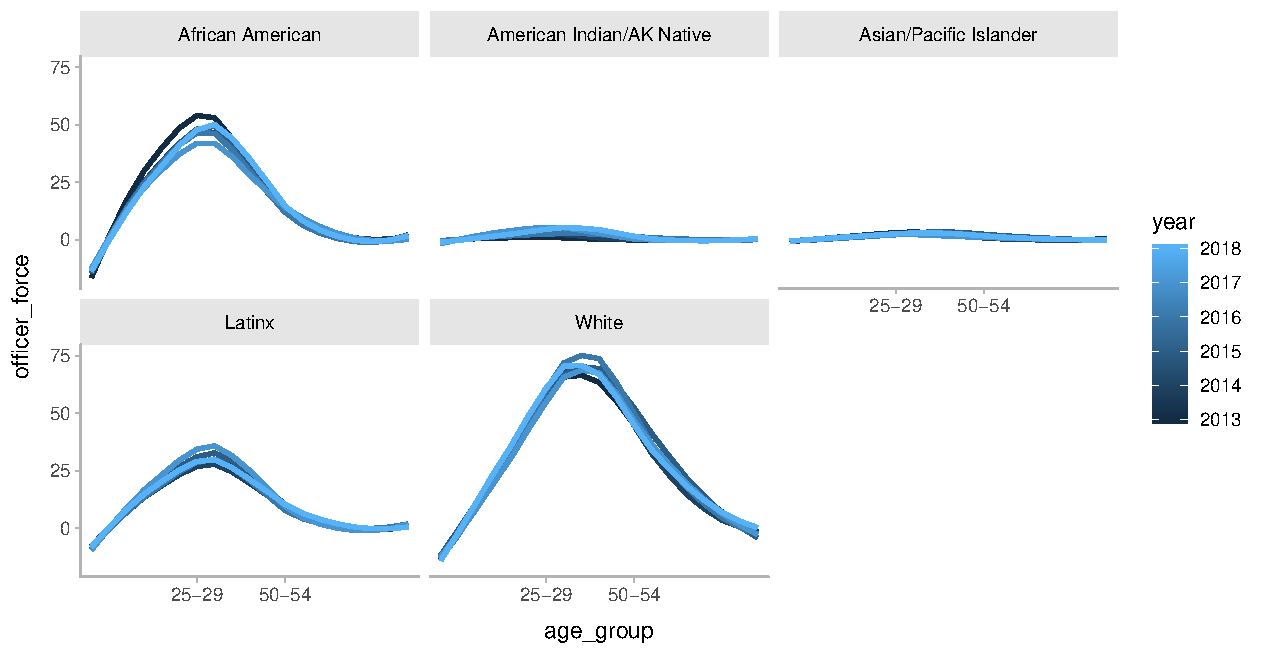
\includegraphics[width = \linewidth]{vis/fig_a2.pdf}
\caption{Males: Observed count of police-involved deaths by age, race, sex, and year with loess smooth}
\label{fig:a2}
\end{figure}

\begin{figure}
\center
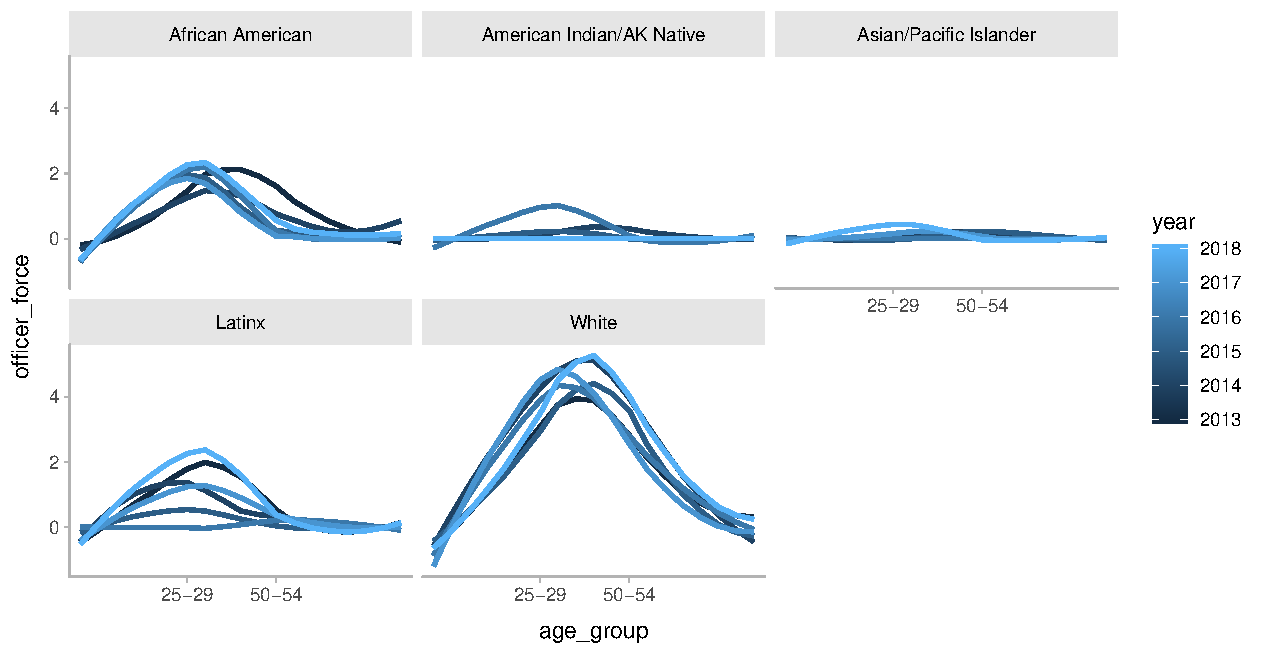
\includegraphics[width = \linewidth]{vis/fig_a3.pdf}
\caption{Females: Observed count of police-involved deaths, by age, race, sex, and year. Note: curves are produced via a loess smooth of the observed data.}
\label{fig:a3}
\end{figure}

Taken together, the observed data suggests that a model allowing intercepts to vary by year could help improve predictions. The observed data also suggest that age, race and sex effects are largely independent of year. While the total count of deaths vary among years, the age, race, and sex patterns observed within each group remains relatively stable across time. 

To further interrogate this assumption about age-effect stability across time, particularly among females, we build stratified regression models that allow for age effects to vary across years. Specially, for each race by gender subset of the data we fit: 1) a model that treats age and year as independent parameters and 2) a model that allows for age slopes to vary across years. 

Results from our stratified models largely confirm the patterns observed in the data. Among males, models that include and exclude a year by age interaction are indistinguishable, both in terms of out of sample accuracy and predicted values. Models for females yielded similar conclusions. Additional tests, which treat year and age as interval measures, modeled via splines, align with these conclusions.  

\subsection*{Simulation models}  

With a better understanding of how time factors into our mortality estimates, we move to build the models that underlie our life-table estimates. We fit and compare four specifications of how race, sex, age and year might predict risk of police-involved mortality. These specification are as follows: 
	\begin{align*}
		M_0\text{:} & \text{ death count} = f(\text{\text{race} + \text{sex} + age} + \text{year}) \\
		M_1\text{:} & \text{ death count} = f([\text{race}*\text{sex}] + \text{age} + \text{year}) \\
    M_2\text{:} & \text{ death count} = f([\text{race}*\text{sex}*\text{age}] + \text{year})   \\
		M_3\text{:} & \text{ death count} = f(\text{age} + [\text{race}*\text{sex}*\text{year}])   
	\end{align*}
Model 0 ($M_0$) assumes that race, sex, age and time have independent effects on mortality risk. Model 1 ($M_1$) allows for race and sex to jointly predict mortality, Model 2 ($M_2$) allows for race and sex effects to vary by age, and Model 3 ($M_3$) allows for race and gender effects to vary by year. All models are multilevel, with race and sex fixed-effects and age-group and year-specific random intercepts specified throughout. Log population size is used as an offset in each model.  

To determine which model best describes the data, we use leave-one-out-cross-validation information criterion (LOO-IC) estimates \cite{vehtari2016bayesian}. LOO-IC estimates are calculated from approximate leave one out cross-validation tests and broadly summarize a model's accuracy in predicting new data relative to other model specifications. Like other information criterion measures, lower LOO-IC values indicate better fitting models. 

\begin{center}
  \begin{tabular}{ccc}
    model & $\text{LOO-IC}$ \\ 
  \hline
    $M_0$ & 2724.8 \\ 
    $M_1$ & 2715.4 \\
    $M_2$ & 2638.6 \\
    $M_3$ & 2715.5 \\
  \hline
  \end{tabular}
  \end{center}
  % \caption{Model LOO-ICs}
  % \label{tab:a1}

Among the model specifications tested, M2 appears to fit the data the best. As such, we simulate from M2. We estimate this model over each imputed dataset, then pool posterior predictions from each model for 4000 hypothetical death counts with each subpopulation held constant at 100,000,000 persons. This method ensures that we generate stable mortality estimates with reasonable uncertainty intervals, even for sub-groups with few observed events or small populations over the period in which Fatal Encounters data is valid. 

\section*{Life table methods}

All estimates mortality risk and rate estimates in the paper are calculated from multiple decrement period life tables \cite{preston_demography:_2000}. These tables take two inputs: 1) counts of age-race-sex specific deaths from the US population in 2017 derived from the NVSS public mortality files and 2) age-race-sex specific predictions of police use-of-force deaths simulated from the regression models described above.  

This method creates a synthetic cohort of 100,000 individuals for each race-sex group, then evaluates how mortality risk would affect the risk of death over the life course if the age-race-sex specific death rates observed in the 2013 - 2018 Fatal Encounters data and overall mortality rates observed in the 2017 NVSS remained constant. 

% latex table generated in R 3.6.1 by xtable 1.8-4 package
% Tue Aug 20 20:51:01 2019
\begin{table}[ht]
\centering
\begin{tabular}{rllrrr}
  \hline
Age & Race & Sex & Total deaths & Use-of-force deaths & Survivors in cohort \\ 
  \hline
  0 & White & Male & 496.29 & 0.01 & 100000.00 \\ 
    1 & White & Male & 104.04 & 0.01 & 99503.71 \\ 
    5 & White & Male & 56.81 & 0.06 & 99399.67 \\ 
   10 & White & Male & 87.17 & 0.04 & 99342.86 \\ 
   15 & White & Male & 319.95 & 1.30 & 99255.69 \\ 
   20 & White & Male & 637.08 & 3.18 & 98935.74 \\ 
   25 & White & Male & 894.65 & 5.62 & 98298.66 \\ 
   30 & White & Male & 1039.69 & 6.13 & 97404.00 \\ 
   35 & White & Male & 1204.78 & 5.60 & 96364.32 \\ 
   40 & White & Male & 1297.84 & 4.54 & 95159.54 \\ 
   45 & White & Male & 1837.68 & 3.83 & 93861.70 \\ 
   50 & White & Male & 2607.33 & 2.99 & 92024.02 \\ 
   55 & White & Male & 4016.77 & 2.32 & 89416.69 \\ 
   60 & White & Male & 5591.27 & 1.24 & 85399.91 \\ 
   65 & White & Male & 7084.67 & 0.92 & 79808.64 \\ 
   70 & White & Male & 10181.83 & 0.62 & 72723.97 \\ 
   75 & White & Male & 12885.66 & 0.30 & 62542.14 \\ 
   80 & White & Male & 15237.63 & 0.20 & 49656.48 \\ 
   85 & White & Male & 34418.85 & 0.17 & 34418.85 \\ 
   \hline
\end{tabular}
\caption{Excerpt of police use-of-force 
                   multiple decrement period lifetable, 
                   synthetic cohort of 100,000} 
\label{tab:life_samp}
\end{table}


Table \ref{tab:life_samp} shows an excerpt of the full life tables we use in the main analysis. It includes a subset of columns in our calculation of white male police use-of-force mortality risk. Using NVSS 2017 total mortality rates, we separately estimate a single decrement period life-table to obtain age-specific mortality rates and estimate overall cohort mortality. Using this period life table, we estimate both age-specific and cumulative rates of police use-of-force deaths, after adjusting for both cross and within age-period mortality by age group. 

We estimate three sets of tables using our model predictions. One at the 5th percentile of the distribution of posterior predictions, one at the median of posterior predictions, and one at the 95th percentile of the distribution of our posterior predictions. All uncertainty intervals reported in the paper reflect these 90 percent uncertainty intervals. 

\section*{Inclusion criteria and mortality estimates}

We emphasize deaths caused by police use-of-force to ensure we capture only those cases in which police action is the direct cause of death. FE includes a broad number of causes of death. After auditing cause-of-death codes to determine which indicated police use-of-force as a proximate cause, we include cases in which the cause of death was coded as: asphyxiated / restrained; beaten / bludgeoned with instrument; chemical agent / pepper spray; gunshot; medical emergency; and tasered. Gunshots account for 91 percent of these cases.

All suicides and other causes of death are excluded from our main analysis. In addition to suicides, these causes include: burned / smoke inhalation; drowned; drug overdose; fell from a height; other; stabbed; undetermined; and vehicle. Vehicle deaths account for nearly all of the non-suicide excluded deaths. Use-of-force deaths account for about two-thirds of all deaths reported in FE. 

\begin{figure}
	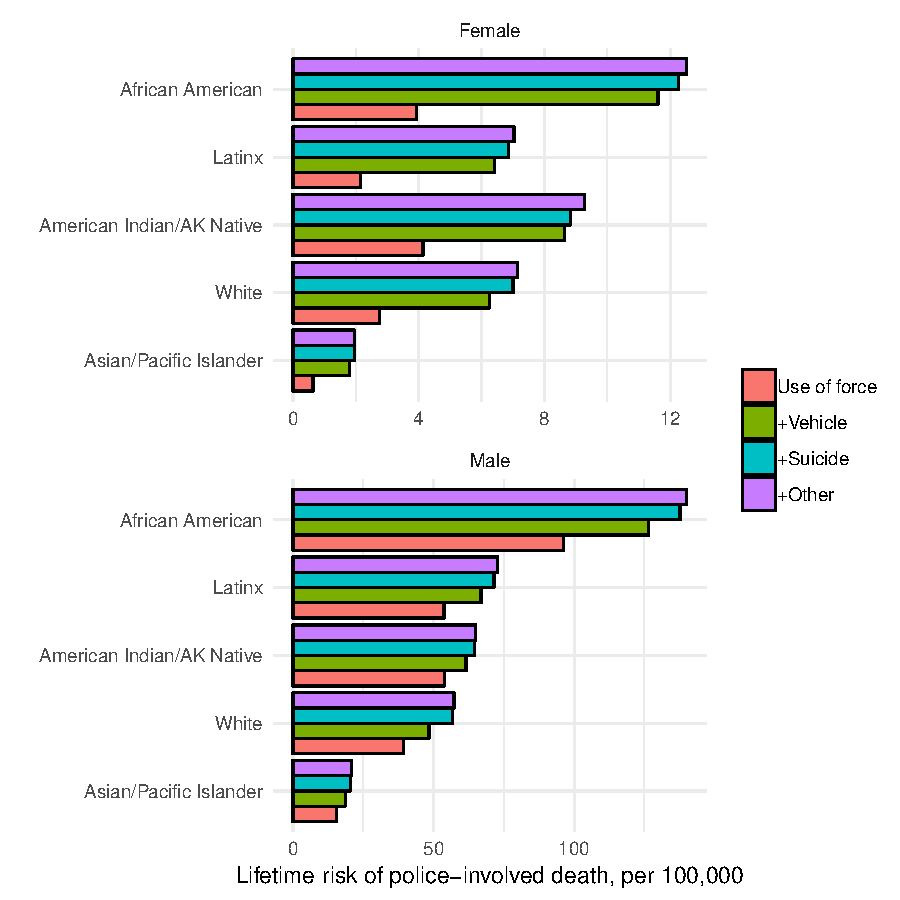
\includegraphics[width=\linewidth]{vis/death_type_c_new.pdf}
	\caption{Cumulative risk of dying during interactions with law enforcement by race, sex, and cause of death}
	\label{fig:death_type}
\end{figure}

We explore the effect that our inclusion criteria have on cumulative mortality estimates by separately estimating lifetime mortality risk for 4 classes of causes of death. Unlike the main analysis, these results are computed from a single imputation of the data, not model-based predictions, and are provided for comparison purposes only as they lack uncertainty estimates. Figure \ref{fig:death_type} shows our estimate of lifetime mortality risk at 2013 - 2018 rates for four nested categories. Use of force deaths; use of force plus vehicle deaths; use of force, vehicle, and suicide deaths; and all reported deaths in FE. 

The greatest impact on mortality estimates is for women. The inclusion of vehicle fatalities more than doubles our estimates of lifetime risk for all racial and ethnic groups. For Black women, our estimates of lifetime risk jump from about 4 in 100,000 when considering only use-of-force deaths to about 12 per 100,000 when including deaths involving motor vehicles. Future research should closely consider how police chases contribute to mortality risk. The inclusion of suicides and other causes of death have much less pronounced effects on our risk estimates.

\bibliography{police_mort}

\end{document}
